\label{Chapter:Design and Procedure of the User Study}
\section{Hypotheses}
\label{section DPUS: Hypotheses}
In Chapter \ref{Chapter:Automated Guided Jumping} we looked at a technique for automated guided navigation using the jumping metaphor and we also saw how the jumps in this technique could be made comprehensible so that the user would know when and where they will jump. The motivations and scenarios that might require such a technique were discussed in Chapter \ref{Chapter:Guided Jumping Motivation}. Keeping in mind the motivation to have a virtual museum that novice \acrshort{vr} users are able to explore we came up with the research questions \cref{rq:rq1}, \cref{rq:rq2} and \cref{rq:rq3} that are mentioned in section \ref{section GJM: Conclusion}.

To study the developed technique with regards to these research questions we decided to design a study that would compare our developed technique for automated guided jumping with a user controlled (free) jumping technique having visual guidance. With this study we hoped to prove the following hypotheses:

\begin{hypothesis}
	\label{hyp:hyp1}
	Participants do not get more simulator sickness while using the automated guided jumping compared to free jumping with visual guidance.
\end{hypothesis}
\begin{hypothesis}
	\label{hyp:hyp2}
	Visual previews before automated jumps will have similar comprehensibility of the jumps compared to free jumping with visual guidance.
\end{hypothesis}
\begin{hypothesis}
	\label{hyp:hyp3}
	Automated guided jumping will reduce task load compared to free jumping with visual guidance.
\end{hypothesis}
\begin{hypothesis}
	\label{hyp:hyp4}
	Users will be able to recall their path when using automated guided jumping as well as when free jumping with visual guidance.
\end{hypothesis}

Hypothesis \cref{hyp:hyp1} is important because we want to justify the need for automate the guided jumping without compromising on the reason for using jumping as the navigation metaphor, that is reduced motion sickness. To also justify that spatial awareness is similar in our technique versus free jumping the study must prove hypothesis \cref{hyp:hyp2} and \cref{hyp:hyp4}. Hypothesis \cref{hyp:hyp2}  also needs to be proved to show that the technique is easy to understand and users will not get confused when using it compared to free jumping. In order to prove the benefit of automated guided jumping over free jumping with visual guidance the study must show that \cref{hyp:hyp3} is true.  

\section{Study Task and Limitations}
\label{section DPUS: Study Task and Limitations}
As the study will be comparing automated jumping with free jumping using visual guiding, it was important to plan a controlled study design such that there would be no other influencing variables besides the automation. Therefore, when developing the free jumping technique that would be used for comparison we had to make sure that the only difference between it and our automated jumping technique would be that the user would make the jumps themselves instead of being automatically moved. There are still nodes and way points in the scene that are used to show visual guidance with an avatar being visible at the next node and a path drawn through way points as in figure \ref{fig:study-free-jumping}. The figure also shows the teleportation indicator with a curve pointing to it that users can use to select the position and orientation they want to be at after the jump.

\begin{figure}[]
	(\centering 1)
	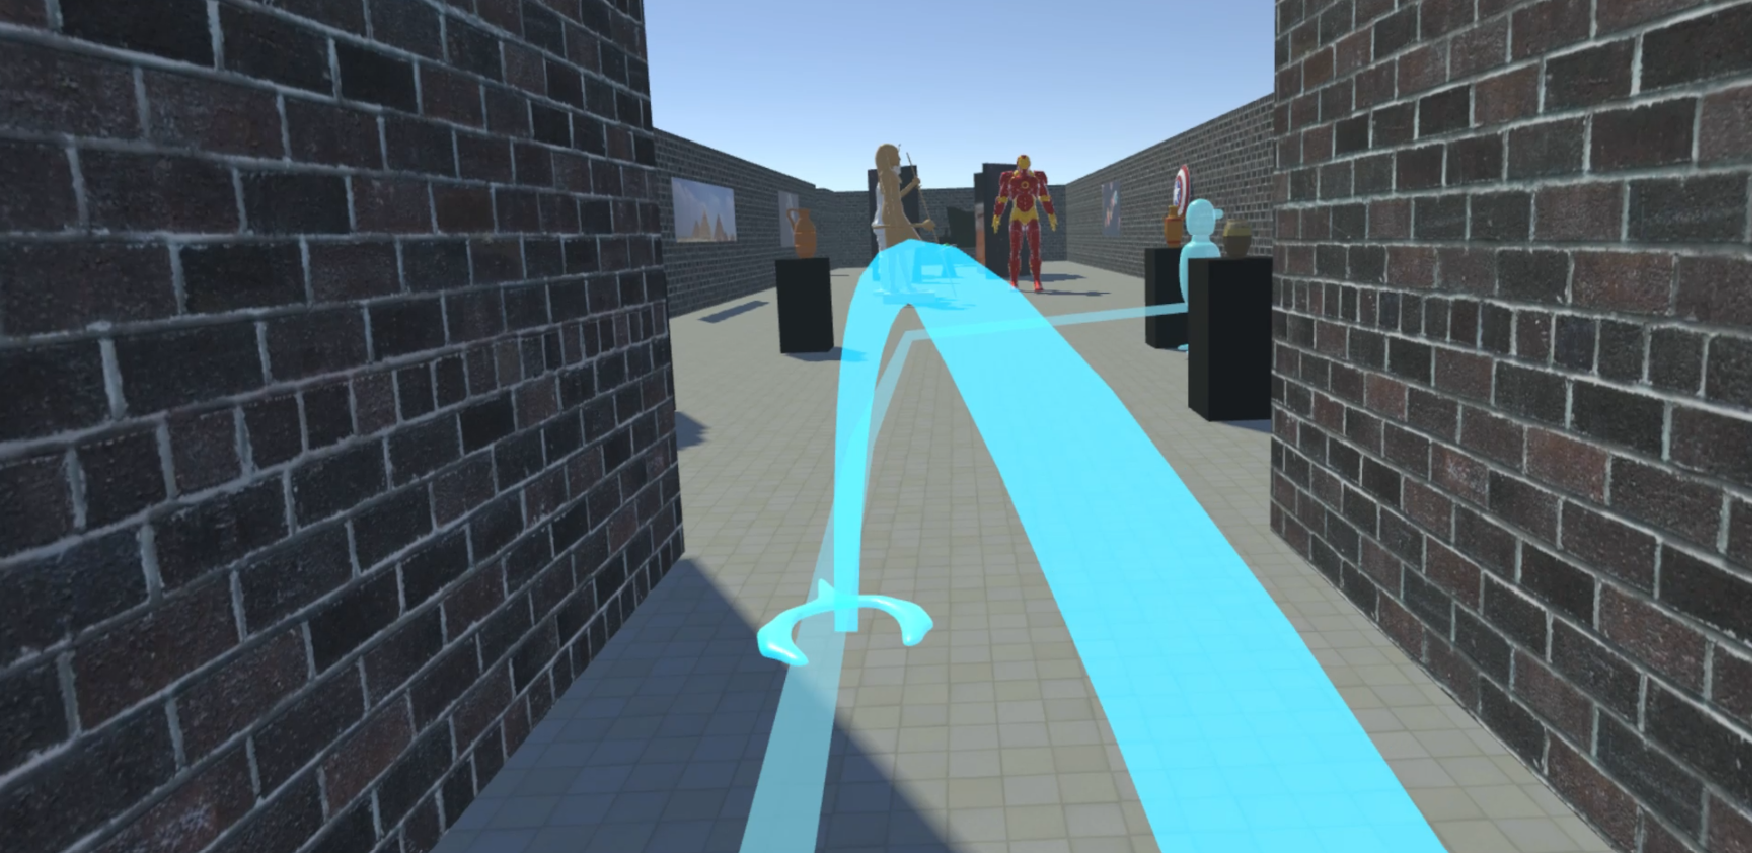
\includegraphics[width=0.25\textwidth]{images/free-jumping.pdf}
	(\centering 2)
	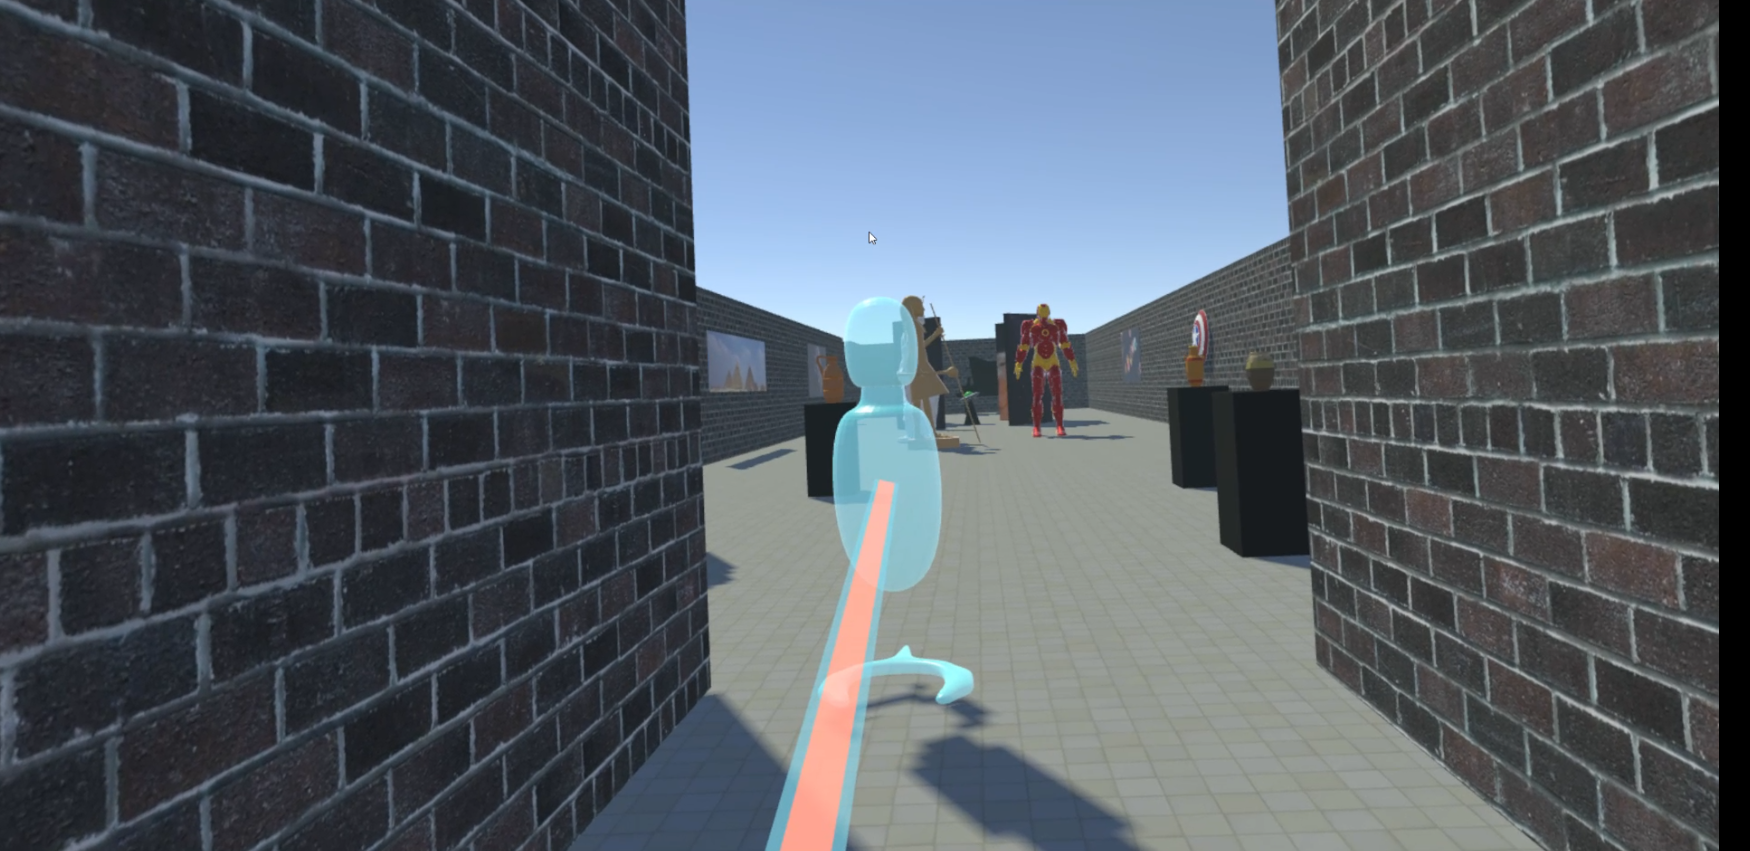
\includegraphics[width=0.25\textwidth]{images/automated-jumping.pdf}
	\caption{Free jumping with visual guidance.}
	\label{fig:study-free-jumping}
\end{figure}

As discussed in \ref{section GJM: Virtual Tours} one of the use cases for guiding techniques is virtual tours and we developed our technique for such a scenario as mentioned in section \ref{subsection AGJ ID: Scenario}. Therefore, the study design also kept in mind a virtual tour situation and considered the potential problem situations that may occur and the possible tasks that may be expected when touring through a virtual space. For this study the task was narrowed to touring a virtual museum with exhibits and trying to remember the path taken as well as the objects seen. This is a useful task when going through a museum and gives answers about whether the techniques used are facilitating acquisition of relevant knowledge of the scene as we hoped to do so through our technique and can be seen in our research question \cref{rq:rq1}.

This task situation for this study will not cover all possible situations that may arise when taking a virtual tour such as:
\begin{itemize}
	\item Exhibits that are very close or far from each other.
	\item More than 2 possible paths to choose from at some nodes.
\end{itemize} 

\section{Variables and Conditions}
\label{section DPUS: Variables and Conditions}
Keeping in mind the task of touring a museum and remembering the path and objects, there are certain variables that need to be varied between the two techniques and others that need to be measured. 

\subsection{Independent Variables}
\label{subsection DPUS VC: Independent Variables}
As we saw in section \ref{section DPUS: Study Task and Limitations}, automation is the only variable that should be different between the two techniques that are being compared. This means that one technique will have automated jumping and the other will not but the visual guidance and ability to have a choice must remain the same. In addition it is important to keep the number of nodes and way points the same. It is also necessary to keep the environment and objects of similar complexity. 

\subsection{Dependent Variables}
\label{subsection DPUS VC: Dependent Variables}
The variables that would depend on whether the technique is automated or not are related to the hypothesis that we introduced in section \ref{section DPUS: Hypotheses}. The amount of simulator sickness needs to be measured somehow to answer hypothesis \cref{hyp:hyp1}. A higher amount of simulator sickness is undesirable while lower amounts are better. Hypotheses \cref{hyp:hyp2} can only be answered by finding some way to determine comprehensibility of jumps. The more comprehensible users find a jump the better. The variable needed to answer hypothesis \cref{hyp:hyp3} is the task load that users feel they had. A lower task load means that users felt they had to make less effort to complete their task and is, therefore, better. Finally, we also need to measure path recall so that we can prove hypothesis \cref{hyp:hyp4}. The more a user is able to recall their path the better. We will look into details on how these variables are extracted during the study in section \ref{section DPUS: Study Procedure}.

\subsection{Study Conditions}
\label{subsection DPUS VC: Study Conditions}
Since we have two techniques to be compared we decided to go with a within user design with 2 study conditions, one using the automated guiding and the other using free jumping with guidance. To avoid participants recall of the environment after the first condition effecting their recall of the environment for the second condition, it is necessary to have two different but comparable scenes. In addition, to avoid the environment or the study order impacting the results the techniques we decided to alternate the order of the conditions while keeping the environment order the same each time.  
 
\section{Study Procedure}
\label{section DPUS: Study Procedure}
In the previous section we defined variables and conditions for the study. Based on these we planned the study procedure which we will now outline in this section starting with the study setup followed by the study plan.

\subsection{Study Setup}
\label{subsection DPUS SP: Study Setup}
The study setup can be divided into three parts which we will discuss in this section. The hardware setup within a physical space, the virtual environment setup and the user feedback.

\subsubsection{Hardware}
\label{subsubsection DPUS SP SS: Hardware}
As we implemented the technique using hand tracking for the Oculus Quest 2, the study was conducted using this \acrshort{hmd}. The Quest 2 has Oculus Insight technology, which tracks changes in the users' position and orientation without need for external tracking. The play space was set to stationary so that users could remain seated while doing the task as there was no need for physical movement. However, to ensure participants could physically rotate, a revolving chair was setup for them to sit on rather than a stationary one. The participants were also equipped with the Oculus Quest 2 controllers but they only needed to make use of the right controller for the free jumping technique and did not need to use a controller for the automated jumping. The environment was displayed per eye at a resolution of 1832×1920 pixels and with a refresh rate of approximately 72 Hz. The headset was connected with a USB cable through Oculus Link, to a computer running the virtual environment on Unity. An additional laptop computer was also setup so that participants could answer question on it in between the tasks and at the end of the study. There was also some space on the desks with a paper for a drawing task for the path recall, which will be explained more in section \ref{subsection DPUS SP: Study Plan} and is linked in Appendix \ref*{Appendix:Questionnaire}. Finally, the experimenter controlled study conditions via the keyboard connected to the workstation running the environment on Unity. Figure ref shows a drawing of the physical study environment and setup.
 
\subsubsection{Virtual Environment}
\label{subsubsection DPUS SP SS: Virtual Environment} 
More than one virtual environment was used for the study. These could be divided into rooms between which the user would switch once each part of the study was conducted. There was one tutorial room in which tutorials for both techniques would take place. There were then two other rooms which were the actual environment for the study tasks. These rooms were a simple museum setup with three rooms connected by one T-shaped corridor and two simple corridors. The rooms had a number of exhibits with a total of 11. There were also 13 paintings distributed along the walls of the rooms and corridors. Top down views of these three rooms can be seen in figure \ref{fig:study-environment}. Room B is a mirror of Room A but has different exhibits and paintings.

\begin{figure}[]
	(\centering 1)
	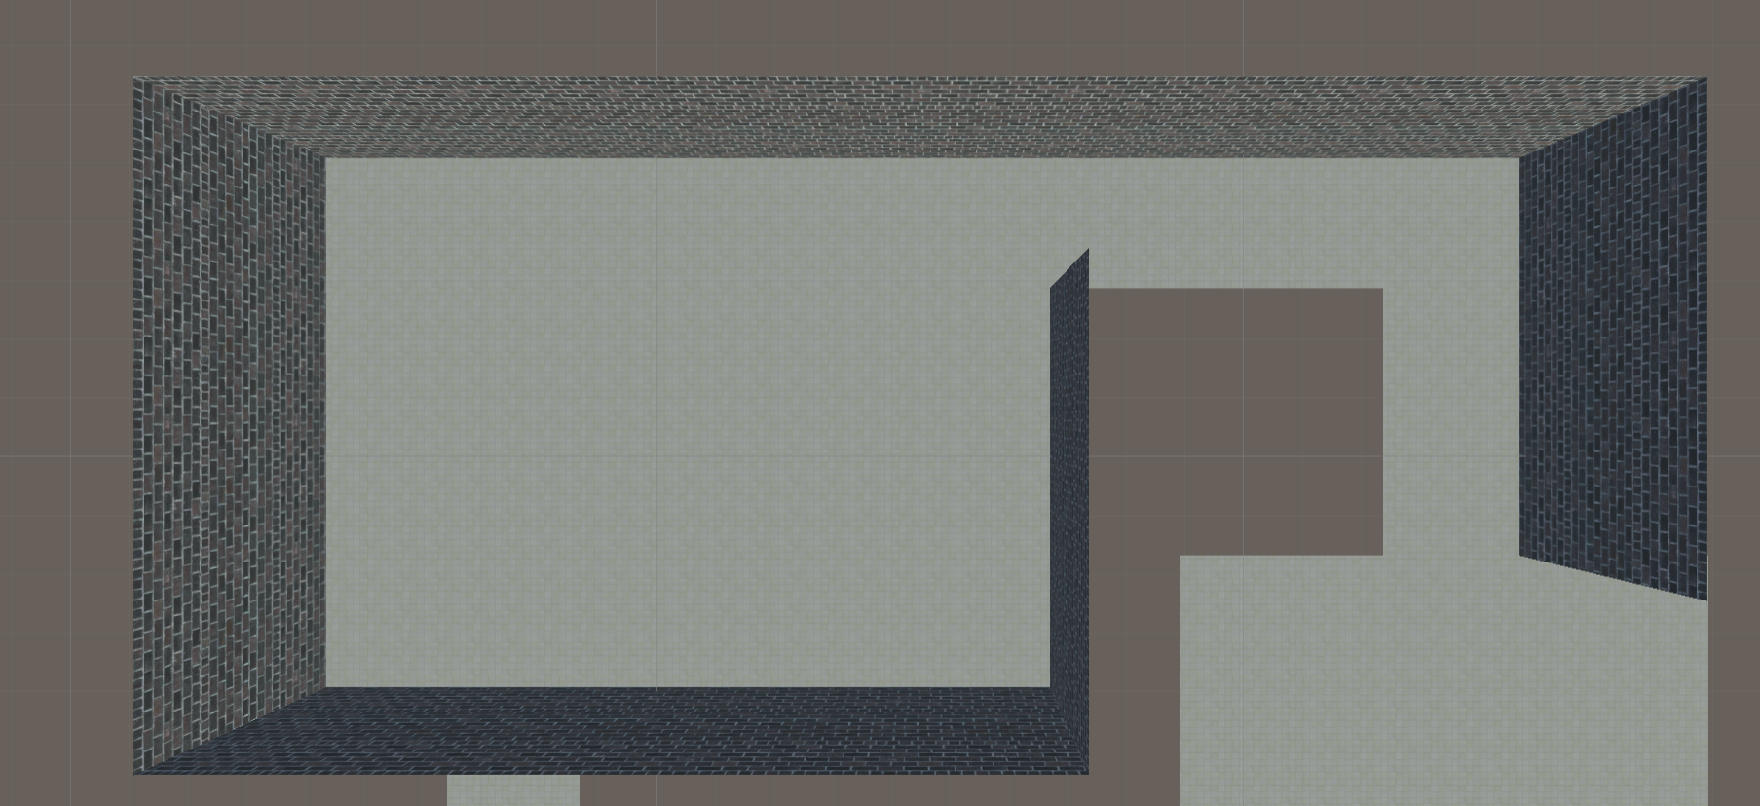
\includegraphics[width=0.25\textwidth]{images/tutorial-room.pdf}
	(\centering 2)
	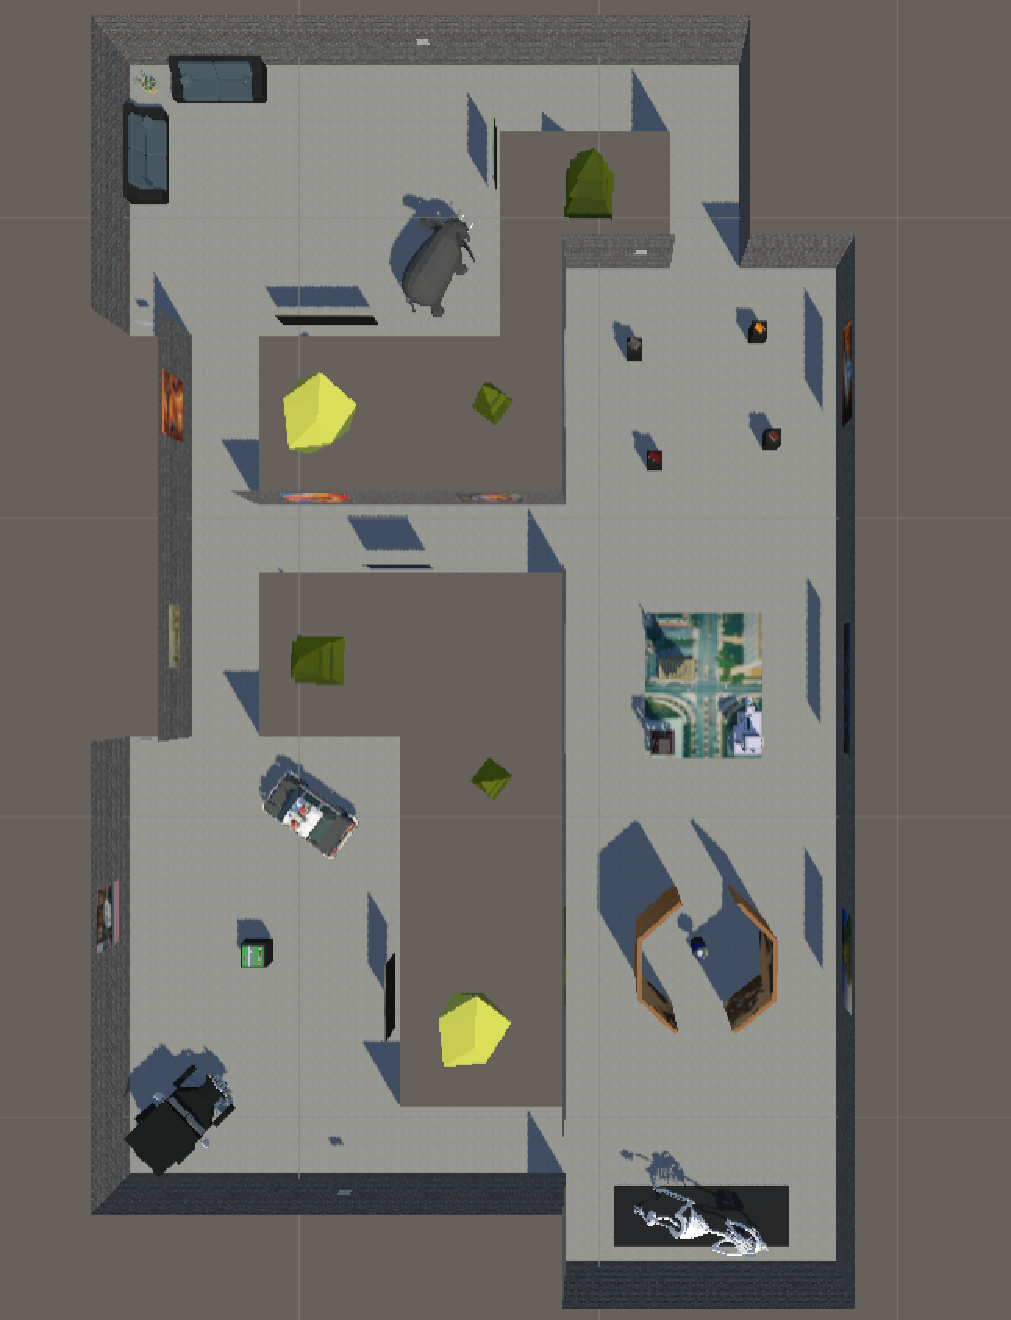
\includegraphics[width=0.25\textwidth]{images/museum-1-objects.pdf}
	(\centering 3)
	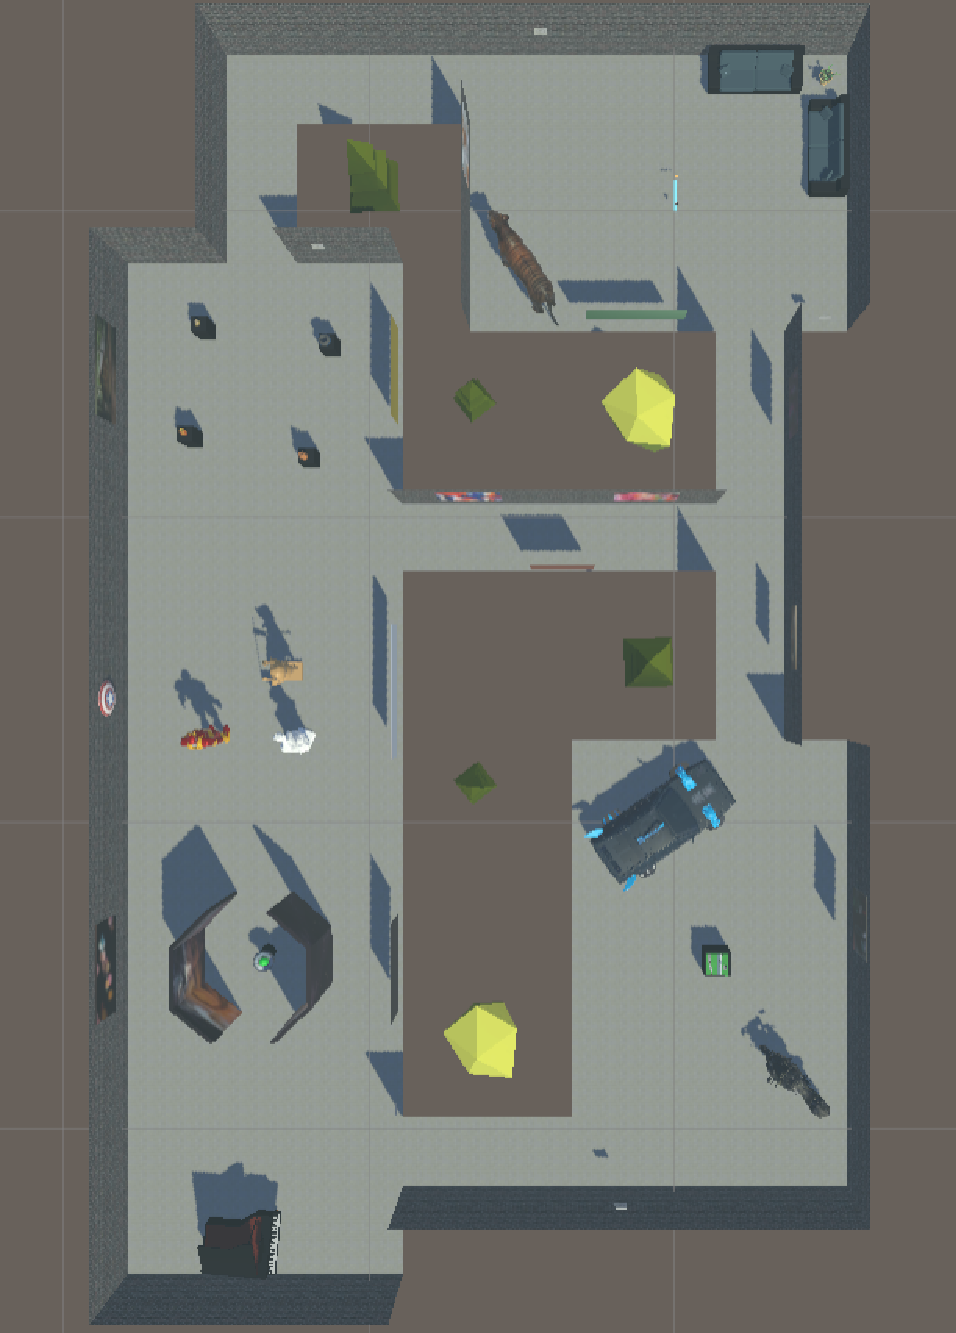
\includegraphics[width=0.25\textwidth]{images/museum-2-objects.pdf}
	\caption{The virtual rooms used for the study with a (1) Tutorial room, (2) Room A and (3) Room B.}
	\label{fig:study-environment}
\end{figure}

\subsection{Study Plan}
\label{subsection DPUS SP: Study Plan}
We explained the study setup in section \ref{subsection DPUS SP: Study Setup} and now we will see the study plan. Before the study was even conducted participants were emailed with the details of the study and asked for consent to be sent over email. Due to the Covid-19 pandemic, certain precautions had to be given in the email as well. The exact draft of the email can be found in Appendix ref*. Once the participants arrived the study could begin in the order shown in figure ref. The steps shown in this diagram will be explained further in this section. Before and after the study all hardware and stationary that the participant would use was sanitized in accordance with Covid-19 hygiene guidelines. The experimenter also wore a mask during the study.

\subsubsection{Tutorial and Tasks}
\label{subsubsection DPUS SP SP: Tutorial and Tasks}
When participants arrived they were seated in the chair where they would remain for the duration of the study. Then they were once again reminded of what they are consenting to before beginning an audio and screen recording. Participants were also reminded that they could stop the study at any time. They were then given a short briefing on the study process and told that they would begin with a tutorial on two techniques and then carry out two tasks with a questionnaire in between and at the end of these tasks. They also entered some demographic information to the questionnaire before beginning.

Before wearing the headset participants were shown the hand gestures that would need to be used as well as the button on the controller that they would need. The hand gestures were called name thumbs up, hand up and pointing. The controller button used would be the trigger button on the right hand controller. Gesture and button mapping are shown in figure ref. Then the user could wear the Oculus Quest 2 and begin with the study tasks. The study started with a tutorial that was divided in two parts for the two techniques with the order they were presented in depending on the study order that they would be following. There were two possible study orders that could be followed. Automated guiding in the first task and free jumping in the second or vice versa. The tutorials would also be presented in this order. The study orders were alternated between participants. The participants could repeat the tutorials for each technique till they were comfortable with it. The time taken for each tutorial was also recorded. 

Once participants completed both the tutorials they could begin with the tasks. Each task was the same except for the technique and environment. Participants were told to use the technique to move through the environment. They could pause when necessary and look around at objects. When presented with a choice between 2 nodes they could pick whichever node they wanted. They were informed that they would need to draw their path and what they saw and therefore they should try and pay attention to where they were going. As participants moved through the environment their time, positions and orientations were recorded into a log file on every move and any time they paused or had to make a choice. When they chose a node the selected node was also logged. Example logging data is shown in Appendix ref* to show the format.

\subsubsection{Questionnaire}
\label{subsubsection DPUS SP SP: User Feedback}
In between tasks participants could take off their headset and go to the second computer to answer some questions and draw their path. The questions for each task were the same. Finally at the end of the study participants answered some final study questions about both techniques. The exact questions in the questionnaire can be seen in Appendix ref*.

The demographic questions obtained from the questionnaire were age and gender. The intermediate questions used for the study included a question on simulator sickness which was introduced by Fernandes et al. to give a discomfort score~\cite{Fernandes2016}. Then the participants were also asked their perceived level of comfort and their reasons.

To measure the task load we decided to use the NASA \acrfull{tlx} as introduced by Stanton et al. as a method for mental workload assessment~\cite{Stanton2005}. We then had some questions about the technique used to get information regarding the comprehensibility of jumps. The questions were both quantitative and qualitative to get a clear understanding on what the participants understood about the technique and whether they were confused at any point about their position and orientation. After the task questions were answered participants had to draw the objects they saw and their paths on a provided map, which was a top down view of the room without any objects in it. This map can be seen in the Appendix ref*.

Finally, after participants answered questions for Task B there were some final study questions to get quantitaive feedback on the participants preferred technique and the reasons for it, as well as additional feedback on what they liked about each technique, what situations they would prefer it in and any other feedback about the techniques. This allowed us to have a more holistic view of the experience the users had with each technique.



